\section{Durchführung}
\label{sec:Durchführung}

\subsubsection{Untersuchung der Amplitude und Berechnung des Dämpfungwiderstandes}

Zur Untersuchung der Zeitanhängigkeit der Amplitude und zur Berechnung des Dämpfungwiderstandes
wird ein gedämpfter Schwingkreis gemäß Abbildung \ref{fig:gsk2} aufgebaut. Dieser wird mit einem
Nadelimpulsgenerator so angeregt, dass zwischen zwei Impulsen die Amplitude um den Faktor drei 
bis acht abgenommen hat. Weiterhin soll der kleinere der beiden Festwiderstände verwendet werden
und um Abweichungen der Messungen durch andere Bauteile zu vermeiden, wird ein hochohmiger 
Tastkopf mit $R_i = 10\, \si{\mega\ohm}$ verwendet.

\begin{figure}[H]
  \centering
  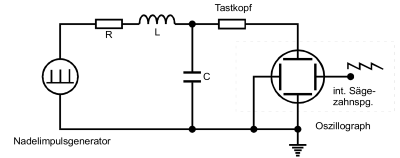
\includegraphics{content/aufgabeA.png}
  \caption{Schaltskizze eines gedämpften Schwingkreises zur Berechnung des Dämpfungwiderstandes und zur Untersuchung der Zeitanhängigkeit der Amplitude}
  \label{fig:gsk2}
\end{figure}
\noindent
Das Bild des Spannungsverlaufs auf dem Oszilloskop soll aufgenommen werden und anschließend soll
zur Bestimmung des Dämpfungwiderstandes $R_{eff}$, sowie der Abklingdauer $T_{ex}$ die Kondensatorspannung
$U_C$ gegen die Zeit aufgetragen werden. Der errechnete Wert von $R_{eff}$ soll anschließend mit dem
tatsächlichen Wert $R$ aus der Schaltung verglichen werden.



\subsubsection{Berechung von dem Widerstand $R_{ap}$}

Die Schaltung wird gemäß Abbildung \ref{fig:gsk3} aufgebaut, wobei der regelbare Widerstand zunächst
auf seinen Maximalwert eingestellt werden soll. Mit diesen Einstellungen ist auf dem Oszilloskop
lediglich das Relaxationsverhalten des Schwingkreises zu erkennen. Um den Dämpfungswiderstand 
zu finden, bei dem der aperiodische Grenzfall eintritt, wird der regelbare Widerstand nun vorsichtig
verkleinert, bis eine Überschwingung, das bedeutet $\frac{\mathrm{d}U_C}{\mathrm{d}t} > 0$, eintritt.
Wird dies erreicht, so muss der regelbare Widerstand gerade so erhöht werden, dass die Überschwingung
verschwindet. Der experimentell gemessene Wert soll anschließend mit dem Theoriewert verglichen werden.

\begin{figure}[H]
  \centering
  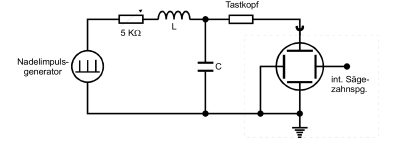
\includegraphics{content/aufgabeB.png}
  \caption{Schaltskizze eines gedämpften Schwingkreises zur Berechnung des Dämpfungwiderstandes $R_{ap}$}
  \label{fig:gsk3}
\end{figure}


\subsubsection{Frequenzabhängigkeit der Kondensatorspannung}

Zunächst wird eine die Schaltung gemäß der Skizze \ref{fig:gsk4} aufgebaut. Um die Frequenzabhängigkeit 
der Kondensatorspannung nun zu messen, wird wieder ein Tastkopf verwendet, da so Störungen, die vom Widerstand
des Millivoltmeters ausgehen zu minimieren. Weiterhin soll der größere der beiden Widerstände verwendet werden.
Nun soll die Erregerspannung $U$, sowie die Kondensatorspannung $U_C$ in Abhängigkeit von der Frequenz $\nu$
gemessen werden. Anschließend soll das Verhältnis der Spannungen halblogarithmisch gegen die Frequenz aufgetragen werden.
Zusätzlich soll der Bereich um die Resonanzfrequenz linear dargestellt werden. Es sollen die Güte $q$ des
Schwingkreises, ebenso wie die Breite vermessen werden. Die Ergebnisse sollen mit den Theoriewerten 
verglichen werden. Der Innenwiderstand des Sinus-Generators darf hierbei nicht vernachlässigt werden.

\begin{figure}[H]
  \centering
  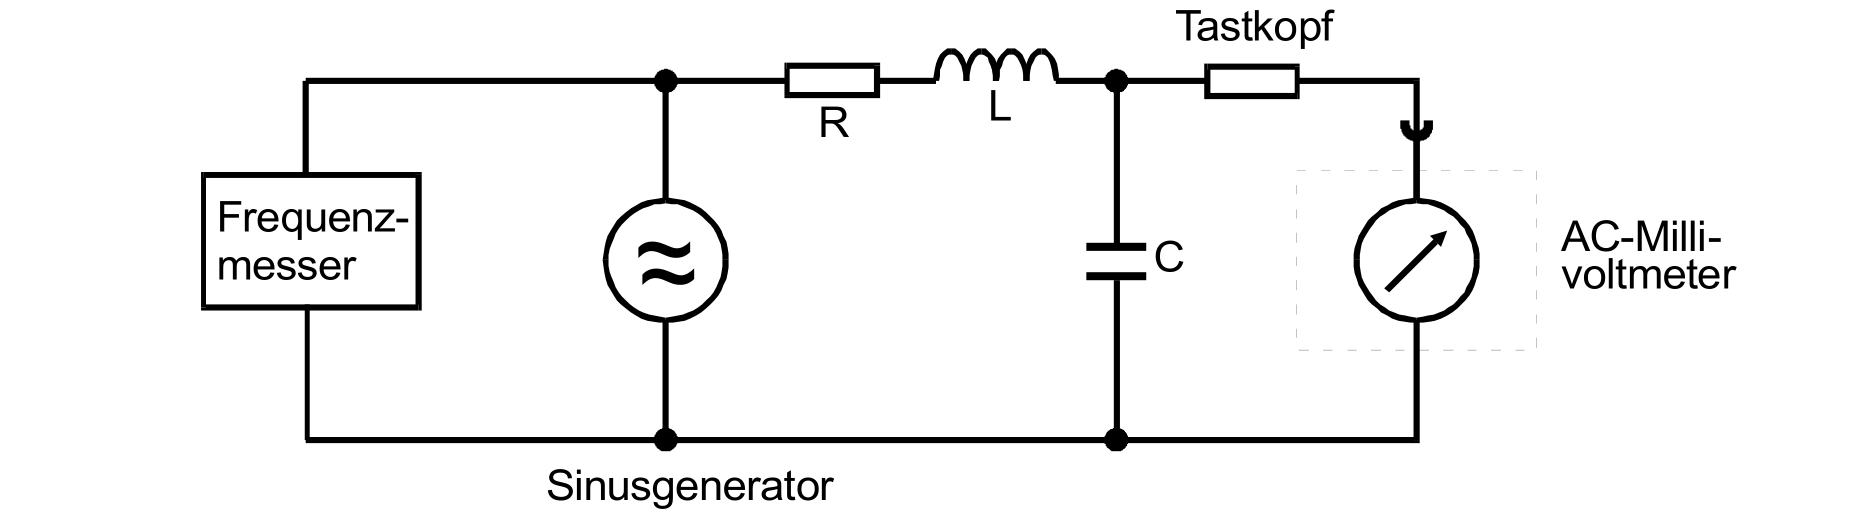
\includegraphics{content/aufgabeC.png}
  \caption{TTTTTTTTTTTTTTTTTTEEEEEEEEEEEEEEEEEEEEEEXXXXXXXXXXXXXXXXXXXXXTTTTTTTTTTTTTTTTTTTTTT}
  \label{fig:gsk4}
\end{figure}


\subsubsection{Frequenzabhängigkeit der Phasenverschiebung}

In diesem Teil des Versuchs soll die Abhängigkeit der Phasenverschiebung von der Frequenz untersucht werden.
Dazu soll eine Schaltung, wie in der Schaltskizze \ref{fig:gsk5} dargestellt ist, aufgebaut werden.



WAS GENAU SOLL ICH MACHEN????

Die gemessenen Werte von der Phasenverschiebung $\phi$ soll halblogarithmisch gegen die Frequenz $\nu$
aufgetragen werden, wobei der Bereich um $\phi = \frac{\pi}{2}$ linear dargestellt werden soll.
Die Resonanzfrequenz $\nu_{res}$ sollen ebenso wie $\nu_1$ und $\nu_2$ bestimmt werden und anschließend
mit den Theoriewerten verglichen werden. 

\begin{figure}[H]
  \centering
  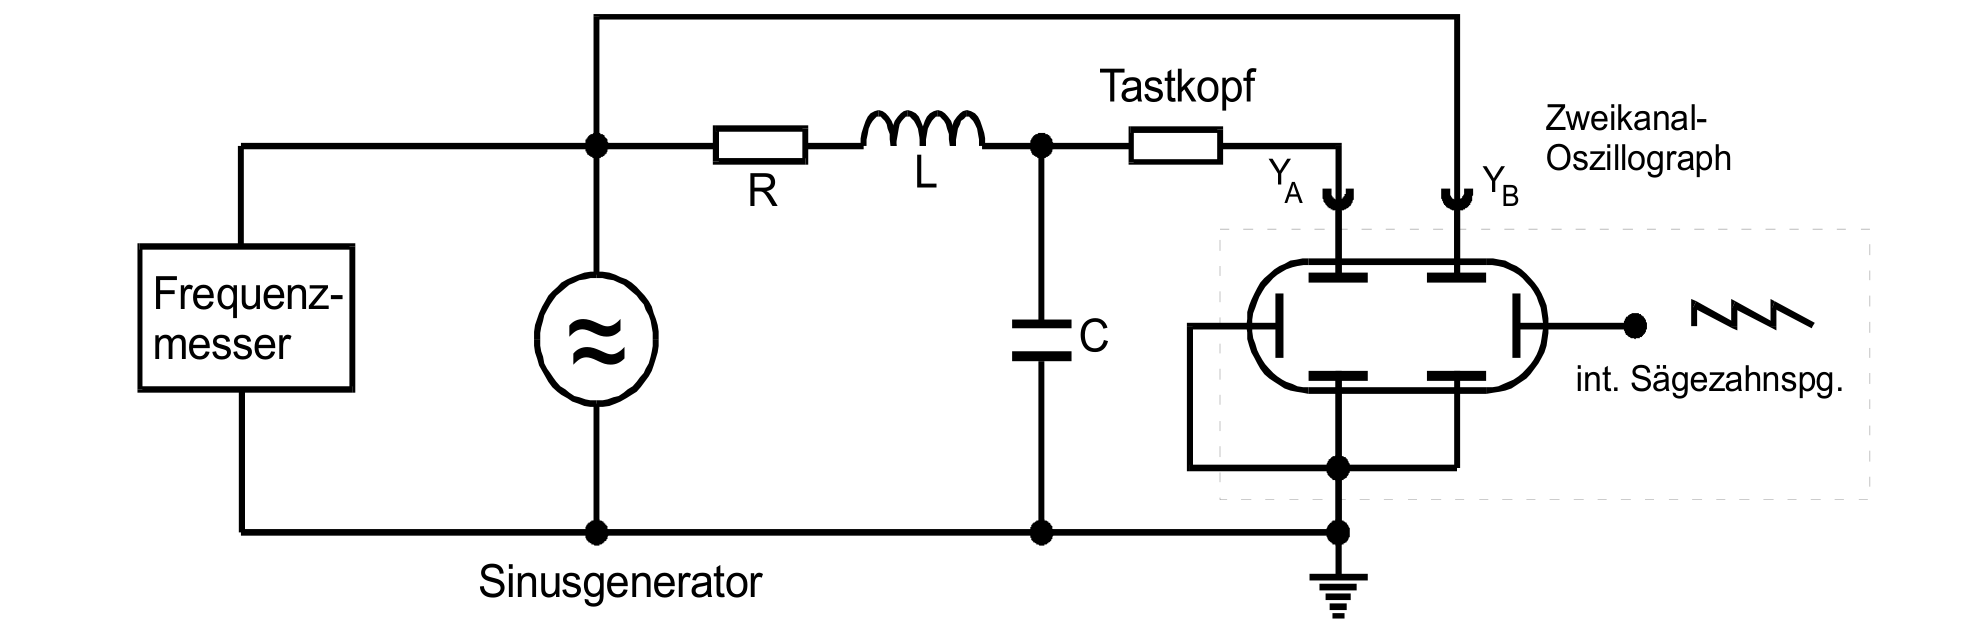
\includegraphics{content/aufgabeD.png}
  \caption{TTTTTTTTTTTTTTTTTTEEEEEEEEEEEEEEEEEEEEEEXXXXXXXXXXXXXXXXXXXXXTTTTTTTTTTTTTTTTTTTTTT}
  \label{fig:gsk5}
\end{figure}
